%%%%%%%%%%%%%%%%%%%%%%%%%%%%%%%%%%%%%%%%%%%%%%%%%%%%%%%%%%%%%%%%%%%%%%%%%%%% 
% !TEX root =  free221.tex
% Time-stamp : 9/10/2012 1:55:27 PM
%%%%%%%%%%%%%%%%%%%%%%%%%%%%%%%%%%%%%%%%%%%%%%%%%%%%%%%%%%%%%%%%%%%%%%%%%%%% 
\chapter{Numbers and Functions}


The subject of this course is ``functions of one real variable'' so we
begin by wondering what a real number ``really'' is, and then, what a
function is.

\section{What is a number?}

\subsection{Different kinds of numbers}
The simplest numbers are the \emph{positive integers}
\[
1, 2, 3, 4,\cdots
\]
the number \emph{zero}
\[
0,
\]
and the \emph{negative integers}
\[
\cdots,-4, -3, -2, -1.
\]
Together these form the integers or ``whole numbers.''

Next, there are the numbers you get by dividing one whole number by another
(nonzero) whole number.  These are the so called fractions or \emph{rational
  numbers} such as
\[
\frac 12,\, \frac13,\, \frac23,\, \frac 14,\,\frac24,\,
\frac34,\, \frac43,\, \cdots
\]
or
\[
-\frac 12,\, -\frac13,\, -\frac23,\, -\frac 14,\,-\frac24,\,
-\frac34,\, -\frac43,\, \cdots
\]
By definition, any whole number is a rational number (in particular zero is a
rational number.)

You can add, subtract, multiply and divide any pair of rational numbers and the
result will again be a rational number (provided you don't try to divide by
zero).

One day in middle school you were told that there are other numbers besides the
rational numbers, and the first example of such a number is the square root of
two.  It has been known ever since the time of the greeks that no rational
number exists whose square is exactly 2, i.e.\ you can't find a fraction $\frac
mn$ such that
\[
\bigl(\frac mn\bigr)^2 = 2, \text{ i.e. }
m^2= 2n^2.
\]

\marginpar{%
  Finding $\sqrt{2}$\,:\rule[-4pt]{0pt}{1pt}\\
  \begin{tabular}{r@{.}lr@{.}ll}
    \toprule
    \multicolumn{2}{c}{$x$}&
    \multicolumn{2}{c}{$x^2$}\\ \midrule
    1&2 & 1&44\\
    1&3 & 1&69\\
    \bfseries\itshape1&\bfseries\itshape4 & \bfseries\itshape1&\bfseries\itshape96&<2\\
    \bfseries\itshape1&\bfseries\itshape5 & \bfseries\itshape2&\bfseries\itshape25&>2\\
    1&6 & 2&56\\
    \bottomrule
  \end{tabular}%
}
Nevertheless, if you compute $x^2$ for some values of $x$ between $1$ and $2$,
and check if you get more or less than $2$, then it looks like there should be
some number $x$ between $1.4$ and $1.5$ whose square is exactly $2$.  So, we
\textit{assume} that there is such a number, and we call it the square root of
2, written as $\sqrt2$.  This raises several questions.  How do we know there
really is a number between $1.4$ and $1.5$ for which $x^2=2$?  How many other
such numbers are we going to assume into existence?  Do these new numbers obey
the same algebra rules (like $a+b = b+a$) as the rational numbers?   If we
knew precisely what these numbers (like $\sqrt2$) were then we could perhaps
answer such questions.  It turns out to be rather difficult to give a precise
description of what a number is, and in this course we won't try to get
anywhere near the bottom of this issue.  Instead we will think of numbers as
``infinite decimal expansions.''

One can represent certain fractions as decimal fractions, e.g.
\[
\frac{279}{25}= \frac{1116}{100} = 11.16.
\]
Not all fractions can be represented as decimal fractions.  For instance,
expanding $\frac13$ into a decimal fraction leads to an unending decimal
fraction
\[
\frac13 = 0.333\,333\,333\,333\,333\,\cdots
\]
It is impossible to write the complete decimal expansion of $\frac13$
because it contains infinitely many digits.  But we can describe the
expansion: each digit is a three. An electronic calculator, which
always represents numbers as \emph{finite} decimal numbers, can never
hold the number $\frac13$ exactly.

Every fraction can be written as a decimal fraction which may or may
not be finite.  If the decimal expansion doesn't end, then it must
repeat.  For instance,
\[
\frac17 = 0.142857\,142857\,142857\,142857\,\dots
\]
Conversely, any infinite repeating decimal expansion represents a
rational number.

A \emph{real number} is specified by a possibly unending decimal
expansion.  For instance,
\[
\sqrt 2 = 1.414\,213\,562\,373\,095\,048\,801\,688\,724\,
209\,698\,078\,569\,671\,875\,376\,9\dots
\]
Of course you can never write \textit{all} the digits in the decimal expansion,
so you only write the first few digits and hide the others behind dots. To
give a precise description of a real number (such as $\sqrt2$) you have to
explain how you could \textit{in principle} compute as many digits in the
expansion as you would like.  During the next three
semesters of calculus we will not go into the details of how this should be
done.

\subsection{A reason to believe in $\sqrt2$}
The Pythagorean theorem says that the hypotenuse of a right triangle with sides
1 and 1 must be a line segment of length $\sqrt2$.
In middle or high school you learned something similar to the following geometric
construction of a line segment whose length is $\sqrt2$.  Take a square with
side of length 1, and construct a new square one of whose sides is the diagonal
of the first square.  The figure you get consists of 5 triangles of equal area
and by counting triangles you see that the larger square  has exactly twice the
area of the smaller square.
\marginpar{%
  
    \begin{picture} (70.000000,70.000000)(0,0)
    \put(0.0, 0.0){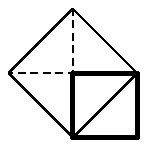
\includegraphics{01smallsquareroot2.pdf}}
    \end{picture}
\\
  \sffamily\footnotesize%
  The big square has twice the area of the small square.}
Therefore the diagonal of the smaller square, being
the side of the larger square, is $\sqrt2$ as long as the side of the smaller
square. 



\subsection{Why are real numbers called real? }
All the numbers we will use in this first semester of calculus are ``real
numbers.'' At some point in history it became useful to assume that there
is such a thing as $\sqrt{-1}$, i.e.~a number whose square is $-1$.  No
real number has this property since the square of any real number is
positive, so it was decided to call this new imagined number ``imaginary''
and to refer to the numbers we already had (rationals, $\sqrt2$-like
things) as ``real.''

\subsection{Reasons not to believe in $\infty$}
\label{sec:infinity-not-a-number}
Calculus is all about infinitely large and infinitely small
quantities.  We will use the symbol $\infty$ (pronounced ``infinity'')
all the time, and the way this symbol is traditionally used would suggest that we
are thinking of $\infty$ as just another number.  But $\infty$ is
different.  The ordinary rules of algebra don't apply to $\infty$.  As
an example of the many ways in which these rules can break down, just
think about ``$\infty + \infty$.''  What do you get if you add
infinity to infinity?  The elementary school argument for finding the
sum is: ``if you have a bag with infinitely many apples, and you add
infinitely many more apples, you still have a bag with infinitely many
apples.'' So, you would think that
\[
\infty + \infty = \infty.
\]
If $\infty$ were a number to which we could apply the rules of
algebra, then we could cancel $\infty$ from both sides, 
\[
\infty + \not\!\!\infty = \not\!\!\infty \implies \infty = 0.
\]
So infinity is the same as zero!  If that doesn't bother you, then
let's go on.  Still assuming $\infty$ is a number we find that
\[
\frac{\infty}{\infty} = 1,
\]
but also, in view of our recent finding that $\infty = 0$, 
\[
\frac{\infty}{\infty} = \frac{0}{\infty} = 0.
\]
Therefore, combining these last two equations,
\[
1=\frac { \infty }{\infty}=0.
\]
In elementary school terms: ``one apple is no apple.''

This kind of arithmetic is not going to be very useful for scientists (or
grocers), so we need to drop the assumption that led to this nonsense,
i.e.\ we have to agree from here on that \footnote{That is not the end of
  the story.  Twentieth century mathematicians have produced a theory of
  ``non standard real numbers'' which includes infinitely large numbers.
  To keep the theory from running into the kind of nonsense we just
  produced, they had to assume that there are many different kinds of
  infinity: in particular $2\times\infty$ is not the same as $\infty$, and
  $\infty\times\infty = \infty^2$ is yet another kind of infinity.  Since
  there are many kinds of infinity in this theory you can't use the single
  symbol ``$\infty$'' because it doesn't say \emph{which} infinitely large
  number you would be talking about.  In this course we will follow the
  traditional standard approach, and assume there are no ``infinitely large
  numbers.'' But if you want to read the version of the theory where
  infinitely large and small numbers do exist, then you should see
  Keisler's calculus text at
  \centerline{\url{http://www.math.wisc.edu/~keisler/calc.html}} }
\begin{center}
 \framebox{ \bfseries
  INFINITY IS NOT A NUMBER!}
\end{center}

\subsection{The real number line and intervals}
It is customary to visualize the real numbers as points on a straight
line.  We imagine a line, and choose one point on this line, which we
call the \emph{origin}.  We also decide which direction we call
``left'' and hence which we call ``right.''  Some draw the number line
vertically and use the words ``up'' and ``down.''

To plot any real number $x$ one marks off a distance $x$ from the
origin, to the right (up) if $x>0$, to the left (down) if $x<0$.

The \emph{distance along the number line} between two numbers $x$ and
$y$ is $|x-y|$.  In particular, the distance is never a negative
number.

\begin{figure}[h]\centering
  
    \begin{picture} (240.000000,39.187500)(0,0)
    \put(0.0, 0.0){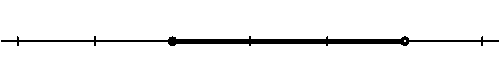
\includegraphics{01drawaninterval.pdf}}
        \put(  6.44,   9.59){\sffamily\itshape $-3$}
    \put( 43.62,   9.59){\sffamily\itshape $-2$}
    \put( 80.81,   9.59){\sffamily\itshape $-1$}
    \put(118.00,   9.59){\sffamily\itshape $0$}
    \put(155.19,   9.59){\sffamily\itshape $1$}
    \put(192.38,   9.59){\sffamily\itshape $2$}
    \put(229.56,   9.59){\sffamily\itshape $3$}
\end{picture}

  \caption{To draw the half open interval $[-1,2)$ use a filled dot to
    mark the endpoint that is included and an open dot for an excluded
    endpoint.  Some like to draw the number line vertical like a
    thermometer.  }
  \label{fig:01drawaninterval}
\end{figure}
\marginpar{\input figures/01drawaninterval-vertical.tex}%

In modern abstract mathematics a collection of real numbers (or any
other kind of mathematical objects) is called a \emph{set}.  Below are
some examples of sets of real numbers.  We will use the notation from
these examples throughout this course.

The collection of all real numbers between two given real numbers form
an interval.  The following notation is used
\begin{itemize}
\item $(a,b)$ is the set of all real numbers $x$ that satisfy $a<x<b$.
\item $[a, b)$ is the set of all real numbers $x$ that satisfy $a\leq x<b$.
\item $(a, b]$ is the set of all real numbers $x$ that satisfy $a< x\leq b$.
\item $[a, b]$ is the set of all real numbers $x$ that satisfy $a\leq x\leq b$.
\end{itemize}
If the endpoint is not included then it may be $\infty$ or $-\infty$.
E.g.\ $(-\infty, 2]$ is the interval of all real numbers (both
positive and negative) that are $\leq 2$.

\begin{figure}[t]\centering
  \input figures/01root2ontheline.tex
  \caption{To find $\sqrt2$ on the real line you draw a square of sides
    $1$ and drop the diagonal onto the real line.}
\end{figure}

\subsection{Set notation}
\label{sec:set-notation}
A common way of describing a set is to say it is the collection of all
real numbers that satisfy a certain condition.  One uses this notation
\[
\setA = \bigl\{ x \mid \text{$x$ satisfies this or that condition}\bigr\}
\]
Most of the time we will use upper case letters in a calligraphic font
to denote sets.  ($\setA$,$\setB$,$\setC$,$\setD$, \dots)

For instance, the interval $(a, b)$ can be described as
\[
(a, b) = \bigl\{x \mid a<x<b\bigr\}
\]
The set 
\[
\setB = \bigl\{x \mid x^2-1>0\bigr\}
\]
consists of all real numbers $x$ for which $x^2-1>0$, i.e.\ it consists of all
real numbers $x$ for which either $x>1$ or $x<-1$ holds.  This set consists of
two parts: the interval $(-\infty, -1)$ and the interval $(1, \infty)$.

You can try to draw a set of real numbers by drawing the number line and
coloring the points belonging to that set red, or by marking them in some other
way.

Some sets can be very difficult to draw.  For instance, 
\[
\setC = \bigl\{x \mid \text{$x$ is a rational number}\bigr\}
\]
can't be accurately drawn.  In this course we will try to avoid such sets.

Sets can also contain just a few numbers, like
\[
\setD = \{1, 2, 3\}
\]
which is the set containing the numbers one, two and three.  Or the set
\[
\setE = \bigl\{x \mid x^3-4x^2+1 = 0\bigr\}
\]
which consists of the solutions of the equation $x^3-4x^2+1=0$.
(There are three of them, but it is not easy to give a formula for the
solutions.)

If $\setA$ and $\setB$ are two sets then \emph{the union of $\setA$ and $\setB$}
is the set that contains all numbers that belong either to $\setA$ or to
$\setB$.  The following notation is used
\[
\setA\cup\setB = \bigl\{x \mid
\text{$x$ belongs to $\setA$ or to $\setB$ or both.}\bigr\}
\]
Similarly, the \emph{intersection of two sets $\setA$ and $\setB$} is the set of
numbers that belong to both sets.  This notation is used:
\[
\setA\cap\setB = \bigl\{x \mid
\text{$x$ belongs to both $\setA$ and $\setB$.}\bigr\}
\]
\section{Problems}
\problemfont
\begin{multicols}{2}\setlength{\parindent}{0pt}
\problem What is the $2007^{\textit{th}}$ digit after the period in the expansion
of $\frac17$?
\answer
The decimal expansion of
\[
1/7 = 0.\overline{142857}\,142857\,142857\,\cdots
\]
repeats after 6 digits.  Since $2007 =
334\times6+3$ the $2007^{\textrm{th}}$ digit is the same as the
$3^{\textrm{rd}}$, which happens to be a $2$.
\endanswer

\problem Which of the following fractions have finite decimal expansions?
\[
a=\frac 23, \quad b=\frac 3{25},\quad c=\frac{276937}{15625}.
\]

\problem Draw the following sets of real numbers.  Each of these sets is
the union of one or more intervals.  Find those intervals.  Which of these
sets are finite?

\noindent%
\(\DS\setA = \bigl\{x \mid x^2-3x+2\leq 0\bigr\} \)\\
\(\DS\setB = \bigl\{x \mid x^2-3x+2\geq 0\bigr\}\)\\
\(\DS\setC = \bigl\{x \mid x^2-3x > 3\bigr\} \)\\
\(\DS\setD = \bigl\{x \mid x^2-5>2x\bigr\} \)\\
\(\DS\setE = \bigl\{t \mid t^2-3t+2\leq0\bigr\} \)\\
\(\DS\setF = \bigl\{\alpha \mid \alpha^2-3\alpha+2\geq 0\bigr\}\)\\
\(\DS\setG = (0, 1)\cup (5, 7] \)\\
\(\DS\setH = \bigl( \{1\}\cup\{2,3\} \bigr)\cap (0, 2\sqrt2)\)\\
\(\DS\setQ = \bigl\{\theta \mid \sin\theta=\tfrac12\bigr\} \)\\
\(\DS\setR = \bigl\{\varphi\mid \cos\varphi>0\bigr\}\)

\problem Suppose $\setA$ and $\setB$ are intervals.  Is it always true that
$\setA\cap\setB$ is an interval?  How about $\setA\cup\setB$?



\problem Consider the sets
\[
\setM = \bigl\{x \mid x>0\bigr\} \text{ and }
\setN =  \bigl\{y \mid y>0\bigr\}.
\]
Are these sets the same?
\answer
Yes these are the same sets.  Both sets consist of all positive real
numbers: since they contain exactly the same numbers, they are the
same sets.
\endanswer
\problem \groupproblem
Write the numbers
\begin{gather*}
  x=0.3131313131\dots,\\
  y=0.273273273273\dots\\
  \text{ and }
  z=0.21541541541541541\dots
\end{gather*}
as fractions (i.e.\ write them as $\frac mn$, specifying $m$ and
$n$.)

(Hint: show that $100x=x+31$. A similar trick works for $y$, but $z$
is a little harder.)
\answer
$100x = 31.313131\cdots = 31+x \implies 99x = 31 \implies x =
\frac{31}{99}$.

Similarly, $1000y = 273 + y$ so $y= \frac{273}{999}$.

In $z$ the initial ``$2$'' is not part of the repeating pattern, so
subtract it:  $z = 0.2 + 0.0154154154\cdots$.  Now let
$w=0.0154154154\cdots$.  You get $1000w = 15.4+w = 15\frac25 + w =
\frac{77}{5}+w$. Therefore $w= \frac{77}{5\times 999}$.
From this you get
\[
z = \tfrac15+w = \tfrac15 +  \frac{77}{5\times999} = \frac{1076}{4995}.
\]
\endanswer

\problem \groupproblem\label{ex:no-infinitely-small-numbers}
\subprob In \S\ref{sec:infinity-not-a-number} we agreed that
infinitely large numbers don't exist. Do infinitely small numbers
exist?   In other words, does there exist a \emph{positive} number $x$
that is smaller than $\frac1n$ for all $n=1, 2, 3, 4, \cdots$, i.e.
\begin{gather*}
  0<x<\tfrac{1}{2}, \text{ and }
  0<x<\tfrac{1}{3}, \text{ and } \\
  0<x<\tfrac{1}{4}, \text{ and so on} \cdots?
\end{gather*}

\subprob
Is the number whose decimal expansion after the period consists only
of nines, i.e.
\[
a=0.99999999999999999\dots
\]
the same as the number $1$?  Or could it be that there are numbers
between $0.9999\cdots$ and $1$?  I.e.~is it possible that there is
some number $x$ that satisfies
\[
0.999999\cdots < x < 1 \; ?
\]

\subprob  Here is a very similar question:  is
\[
b=0.3333333333333333333\dots
\]
the same as $\frac13$?  Or could there be a number $x$ with
\[
0.333333\dots <x<\tfrac13 ?
\]

\problem In \S\ref{sec:set-notation} we said that the set
\[
\setC = \bigl\{x \mid \text{$x$ is a rational number}\bigr\}
\]
was difficult to draw.  Explain why.

\end{multicols}

\noproblemfont%

\section{Functions}

\subsection{Dependence}
Calculus deals with quantities that depend on each other.  For
instance, the water temperature $T$ of Lake Mendota, as measured at
the pier near the Memorial Union is a well defined quantity, but it
changes with time.  At each different time $t$ we will find a
different temperature $T$.  Therefore, when we say ``the temperature at
the pier of Lake Mendota,'' we could mean two different things:   

\begin{itemize}
\item On one hand we could mean the ``temperature at some given
  time,'' e.g.~the temperature at 3pm is 68F: here the temperature is
  just a number.  The most common notation for this is $T(3) = 68$, or
  $T(3\textrm{pm}) = 68\textrm{F}$.

\item On the other hand we could mean the ``temperature in general,''
  i.e.~the temperatures at all times.  In that second interpretation
  the temperature is not just a number, but a whole collection of
  numbers, listing \emph{all} times $t$ and the corresponding
  temperatures $T(t)$.
\end{itemize}

So $T(t)$ is a number while $T$ by itself is not a number, but a more
complicated thing.  It is what in mathematics is called a
\emph{function}.  We say that \textit{the water temperature is a
  function of time.}

Here is the definition of what a mathematical function is:

\subsection{Definition}
\itshape
To specify a \emph{function} $f$ you must 
\begin{enumerate}
\item give a \emph{rule} that tells you how to compute the value $f(x)$ of
  the function for a given real number $x$, and:
\item say for which real numbers $x$ the rule may be applied.
\end{enumerate}%
The set of numbers for which a function is defined is called its \emph{domain}.
The set of all possible numbers $f(x)$ as $x$ runs over the domain is called the
\emph{range} of the function.  The rule must be \emph{unambiguous:} the same
$x$ must always lead to the same $f(x)$.
\upshape

\medskip

For instance, one can define a function $f$ by putting $f(x) = \sqrt x$ for all
$x\geq0$.  Here the rule defining $f$ is ``take the square root of whatever
number you're given'', and the function $f$ will accept all nonnegative real
numbers.

The rule that specifies a function can come in many different forms.  Most
often it is a formula, as in the square root example of the previous paragraph.
Sometimes you need a few formulas, as in
\[
g(x) = 
\begin{cases}
  2x & \text{for } x<0 \\
  x^2 & \text{for }x\geq0
\end{cases}
\qquad
\text{domain of $g$} = \text{all real numbers.}
\]
Functions whose definition involves different formulas on different
intervals are sometimes called \emph{piecewise defined functions.}

\subsection{Graphing a function}
You get the \emph{graph of a function} $f$ by drawing all points whose
coordinates are $(x,y)$ where $x$ must be in the domain of $f$ and $y = f(x)$.
\begin{figure}[h]
  \centering
  
    \begin{picture} (240.000000,144.800000)(0,0)
    \put(0.0, 0.0){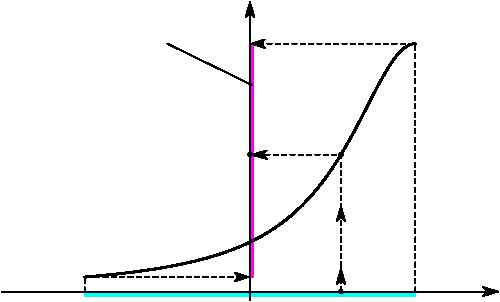
\includegraphics{01graphOFf.pdf}}
        \put( 80.33, 123.97){\sffamily\itshape \makebox[0pt][r]{range of $f$}}
    \put(118.00,  70.71){\sffamily\itshape \makebox[0pt][r]{$y=f(x)$}}
    \put(167.63,  68.71){\sffamily\itshape $(x, f(x))$}
    \put(167.63,   6.97){\sffamily\itshape $x$}
    \put(120.00,  -7.03){\sffamily\itshape \makebox[0pt][c]{domain of $f$}}
\end{picture}

  \caption{The graph of a function $f$. The domain of $f$ consists
    of all $x$ values at which the function is defined, and the range consists
    of all possible values $f$ can have.}
  \label{fig:01graphOFf}
\end{figure}

\begin{figure}[t]
  \centering
  
    \begin{picture} (240.000000,172.000000)(0,0)
    \put(0.0, 0.0){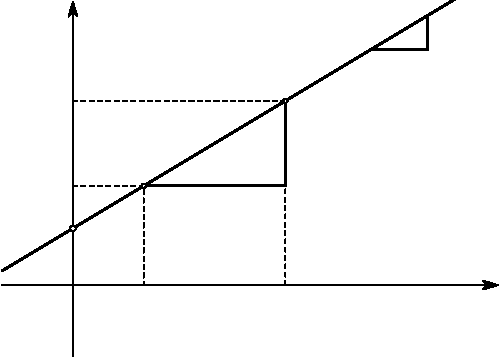
\includegraphics{01line.pdf}}
        \put( 65.00,  90.60){\sffamily\itshape $P_0$}
    \put(133.00, 131.40){\sffamily\itshape $P_1$}
    \put(141.00, 103.00){\sffamily\itshape $y_1-y_0$}
    \put(103.00,  72.60){\sffamily\itshape \makebox[0pt][c]{$x_1-x_0$}}
    \put( 65.00,  23.00){\sffamily\itshape $x_0$}
    \put(133.00,  23.00){\sffamily\itshape $x_1$}
    \put( 25.00,  82.60){\sffamily\itshape $y_0$}
    \put( 25.00, 123.40){\sffamily\itshape $y_1$}
    \put( 33.00,  63.20){\sffamily\itshape \makebox[0pt][r]{$n$}}
    \put(191.40, 139.88){\sffamily\itshape $1$}
    \put(207.00, 155.04){\sffamily\itshape $m$}
\end{picture}

  \caption{The graph of $f(x) = mx+n$ is a straight line.
    It intersects the $y$-axis at height $n$.
    The ratio between the amounts by which $y$ and $x$ increase as you
    move from one point to another on the line is
    $\frac{y_1-y_0}{x_1-x_0} = m$.  This ratio is the same, no matter
    how you choose the points $P_0$ and $P_1$ as long as they are on
    the line.}\label{fig:01line}
\end{figure}
\subsection{Linear functions}
A function $f$ that is given by the formula 
\[
f(x) = mx + n
\]
where $m$ and $n$ are constants is called a \emph{linear function}.  Its graph
is a straight line.  The constants $m$ and $n$ are the \emph{slope} and
\emph{$y$-intercept} of the line.  Conversely, any straight line which is not
vertical (i.e.\ not parallel to the $y$-axis) is the graph of a linear function.
If you know two points $(x_0, y_0)$ and $(x_1, y_1)$ on the line, then then one
can compute the slope $m$ from the ``rise-over-run'' formula
\[
m = \frac{y_1-y_0}{x_1-x_0}.
\]
This formula actually contains a theorem from Euclidean geometry,
namely, it says that the ratio
\[
(y_1-y_0):(x_1-x_0)
\]
is the same for every pair of points $(x_0, y_0)$ and $(x_1, y_1)$
that you could pick on the line.


\subsection{Domain and ``biggest possible domain.'' }
In this course we will usually not be careful about specifying the
domain of a function.  When this happens the domain is understood to
be the set of all $x$ for which the rule that tells you how to
compute $f(x)$ is meaningful.  For instance, if we say that $h$ is the
function 
\[
h(x) = \sqrt x
\]
then the domain of $h$ is understood to be the set of all nonnegative real
numbers
\[
\text{domain of $h$} = [0, \infty)
\]
since $\sqrt x$ is well-defined for all $x\geq 0$ and undefined for $x<0$.

A systematic way of finding the domain and range of a function for which you are
only given a formula is as follows:
\begin{itemize}
\item The domain of $f$ consists of all $x$ for which $f(x)$ is well-defined
  (``makes sense'')
\item The range of $f$ consists of all $y$ for which you can solve the
  equation $f(x) = y$.
\end{itemize}


\subsection{Example -- find the domain and range of $f(x) = 1/x^2$}
The expression $1/x^2$ can be computed for all real numbers $x$ except
$x=0$ since this leads to division by zero.  Hence the domain of the
function $f(x) = 1/x^2$ is
\[
\text{``all real numbers except $0$''}
=\bigl\{x \mid x\neq0\bigr\} = (-\infty, 0)\cup(0, \infty).
\]
To find the range we ask ``for which $y$ can we solve the equation
$y=f(x)$ for $x$,'' i.e.\ for which $y$ can you solve $y=1/{x^2}$ for
$x$?

If $y=1/x^2$ then we must have $x^2 = 1/y$, so first of all, since we
have to divide by $y$, $y$ can't be zero.  Furthermore, $1/y=x^2$ says
that $y$ must be positive.  On the other hand, if $y>0$ then $y=1/x^2$
has a solution (in fact two solutions), namely $x=\pm1/\surd y$.  This
shows that the range of $f$ is
\[
\text{``all positive real numbers''} = \{x \mid x>0\} = (0, \infty).
\]
\subsection{Functions in ``real life.''}
One can describe the motion of an object using a function.  If some
object is moving along a straight line, then you can define the
following function: Let $s(t)$ be the distance from the object to a
fixed marker on the line, at the time $t$.  Here the domain of the
function is the set of all times $t$ for which we know the position of
the object, and the rule is
\begin{center}
  \itshape Given $t$, measure the distance between the object at time $t$ and the
  marker.
\end{center}
\smallskip
\centerline{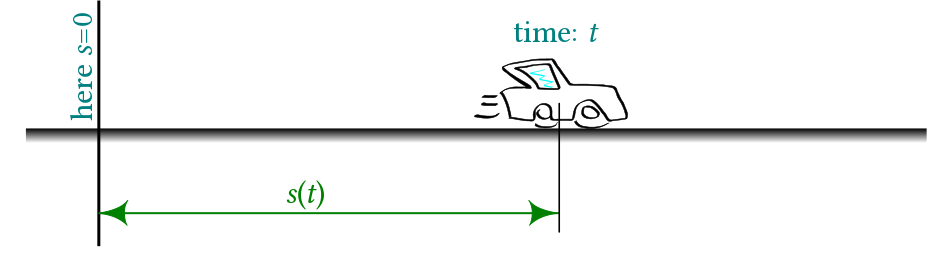
\includegraphics[width=0.6\textwidth]{01car.png}}%
There are many examples of this kind.  For instance, a biologist could
describe the growth of a mouse by defining $m(t)$ to be the mass of the mouse
at time $t$ (measured since the birth of the mouse).  Here the domain is the
interval $[0, T]$, where $T$ is the life time of the mouse, and the rule
that describes the function is
\begin{center}
  \itshape Given $t$, weigh the mouse at time $t$.
\end{center}

\marginpar{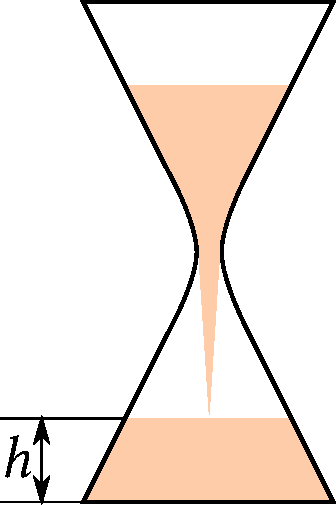
\includegraphics[width=48pt]{01hourglass.pdf}}%
Here is another example: suppose you are given an hourglass.  If you turn
it over, then sand will pour from the top part to the bottom part.  At any
time $t$ you could measure the height of the sand in the bottom and
call it $h(t)$.  Then, as in the previous examples, we can say that the height of
the sand is a function of time.  But in this example you can let the two
variables height and time switch roles: given a value for $h$ you wait
until the pile of sand in the bottom has reached height $h$ and check what
time it is when that happens: the resulting time $t(h)$ is determined by
the specified height $h$.  In this way we can regard time as a function of
height.

\subsection{The Vertical Line Property}
Generally speaking graphs of functions are curves in the plane but
they distinguish themselves from arbitrary curves by the way they
intersect vertical lines: \emph{The graph of a function cannot
intersect a vertical line ``$x=\text{\em constant}$'' in more than one
point}.  The reason why this is true is very simple: if two points lie
on a vertical line, then they have the same $x$ coordinate, so if they
also lie on the graph of a function $f$, then their $y$-coordinates
must also be equal, namely $f(x)$.


\subsection{Example -- a cubic function}
The graph of $f(x) = x^3-x$ ``goes up and down,'' and, even though it
intersects several horizontal lines in more than one point, it
intersects every vertical line in exactly one point.  See
Figure~\ref{fig:01horizontal-and-vertical-line-tests}.

\begin{figure}[t]\centering
  
    \begin{picture} (240.000000,104.000000)(0,0)
    \put(0.0, 0.0){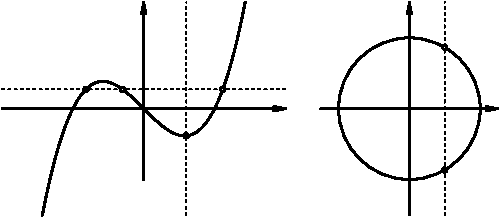
\includegraphics{01cubicANDcircle.pdf}}
        \put( 24.80,   9.50){\sffamily\itshape $y=x^3-x$}
\end{picture}
%
  \caption{The graph of $y=x^3-x$ fails the ``horizontal line test,'' but it
    passes the ``vertical line test.''  The circle fails both tests.}
  \label{fig:01horizontal-and-vertical-line-tests}
\end{figure}

\subsection{Example -- a circle is not a graph}
\label{sec:01circle-izno-graph}
The collection of points determined by the equation $x^2+y^2=1$ is a circle.  It
is not the graph of a function since the vertical line $x=0$ (the $y$-axis)
intersects the graph in two points $P_1(0,1)$ and $P_2(0,-1)$. See again
Figure~\ref{fig:01horizontal-and-vertical-line-tests}.  This example
continues in \S~\ref{sec:implicit-example-h1h2h3} below.


\section{Implicit functions}
For many functions the rule that tells you how to compute it is not an explicit
formula, but instead an equation that you still must solve.  A function that is
defined in this way is called an ``implicit function.''  

\subsection{Example}
We can define a function $f$ by saying that if $x$ is any given number,
then $y = f(x)$ is the solution of the equation
\[
x^2+2y-3=0.
\]
In this example we can solve the equation for $y$, 
\[
y = \frac{3-x^2}2.
\]
Thus we see that the function we have defined is $f(x) = (3-x^2)/2$.

Here we have two definitions of the same function, namely
\begin{itemize}
\item [(i)] ``$y=f(x)$ is defined by $x^2+2y-3=0$,'' and
\item [(ii)] ``$f$ is defined by $f(x) = (3-x^2)/2$.''
\end{itemize}
The first definition is the implicit definition, the second is explicit.
This example shows that with an ``implicit function'' it is not the
function itself, but rather the way it was defined that is implicit.

\subsection{Another example: domain of an implicitly defined function}
Define $g$ by saying that for any $x$ the value $y=g(x)$ is the
solution of
\[
x^2+xy-3=0.
\]
Just as in the previous example you can then solve for $y$, and you
find that
\[
g(x) = y = \frac{3-x^2}x.
\]
Unlike the previous example this formula does not make sense when $x=0$, and
indeed, for $x=0$ our rule for $g$ says that $g(0) = y$ is the solution of 
\[
0^2+0\cdot y-3=0, \text{ i.e. $y$ is the solution of }3=0.
\]
That equation has no solution and hence $x=0$ does not belong to the domain
of our function $g$.  

\begin{figure}[h]
  \centering
  
    \begin{picture} (360.000000,109.400000)(0,0)
    \put(0.0, 0.0){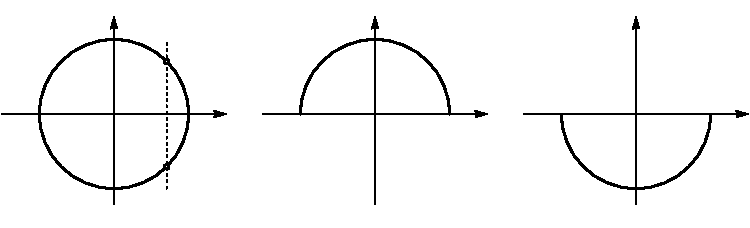
\includegraphics{01circle.pdf}}
        \put( 40.38,  90.50){\sffamily\itshape \makebox[0pt][r]{$x^2+y^2=1$}}
    \put(208.31,  84.01){\sffamily\itshape $y=+\sqrt{1-x^2}$}
    \put(333.61,  23.39){\sffamily\itshape $y=-\sqrt{1-x^2}$}
\end{picture}

  \caption{The circle determined by $x^2+y^2=1$ is not the graph of a
    function, but it contains the graphs of the two functions
    $h_1(x) = \sqrt{1-x^2}$ and $h_2(x)= -\sqrt{1-x^2}$.}
  \label{fig:01circle}
\end{figure}

\subsection{Example: the equation alone does not determine the function}
\label{sec:implicit-example-h1h2h3}
We saw in \S~\ref{sec:01circle-izno-graph} that the unit circle is not
the graph of a function (because it fails the vertical line test).
What happens if you ignore this fact and try to use the equation
$x^2+y^2=1$ for the circle to define a function anyway?
To find out, suppose we define $y=h(x)$ to be ``the solution'' of 
\[
x^2 + y^2=1.
\]
If $x>1$ or $x<-1$ then $x^2>1$ and there is no solution, so $h(x)$ is
at most defined when $-1\leq x\leq 1$.  But when $-1<x<1$ there is
another problem: not only does the equation have a solution, it
has \emph{two} solutions:
\[
x^2+y^2=1 \iff y = \sqrt{1-x^2} \text{ or } y=-\sqrt{1-x^2}.
\]
The rule that defines a function must be unambiguous, and since we
have not specified which of these two solutions is $h(x)$ the function
is not defined for $-1<x<1$.

Strictly speaking, the domain of the function that is defined implicitly by
the equation $x^2+y^2=1$ consists of only two points, namely $x=\pm1$.
Why?  Well, those are the only two values of $x$ for which the equation has
exactly one solution $y$ (the solution is $y=0$.)  To see this in the
picture, look at Figure~\ref{fig:01circle} and find all vertical lines that
intersect the circle on the left exactly once.  

To get different functions that are described by the equation $x^2+y^2=1$,
we have to specify for each $x$ which of the two solutions
$\pm\sqrt{1-x^2}$ we declare to be ``$f(x)$''.  This leads to many possible
choices.  Here are three of them:
\begin{align*}
  h_1(x) & = \text{the non negative solution $y$ of } x^2+y^2=1 \\
  h_2(x) & = \text{the non positive solution $y$ of } x^2+y^2=1 \\
  h_3(x) & = 
  \begin{cases}
    h_1(x) & \text{when $x<0$} \\
    h_2(x) & \text{when $x\geq0$} \\
  \end{cases}
\end{align*}
There are many more possibilities.

\subsection{Why and when do we use implicit functions? Three examples}
\label{sec:why-implicit}
In all the examples we have done so far we could replace the implicit
description of the function with an explicit formula.  This is not always
possible, or, if it is possible, then the implicit description can still be much
simpler than the explicit formula.

As a first example, define a function $f$ by saying that $y=f(x)$ if
and only if $y$ is the largest of the solutions of
\begin{equation}\label{eq:01quadratic-implicit}
  y^2+3y+2x = 0.
\end{equation}
This means that the recipe for computing $f(x)$ for any given $x$ is
``solve the equation $y^2+3y+2x = 0$ for $y$ and set $y$ equal to the
largest solution you find.''  E.g.\ to compute $f(0)$ you set $x=0$
and solve $y^2+3y=0$.  By factoring $y^2+3y = (y+3)y$ you find that
the solutions are $y=0$ and $y=-3$.  Since $f(0)$ is defined to be the
\textit{largest} of the solutions, we get $f(0)=0$.  Similarly, to
compute $f(1)$ you have to solve $y^2+3y +2\cdot1=0$: the solutions
are $y=-1$ and $y=-2$, so $f(1) = -1 $.  For any other $x$ the
quadratic formula tells you that the solutions are
\[
y = \frac{-3 \pm \sqrt{3^2-4\cdot 2x}} {2} = \frac{-3\pm\sqrt{9-8x}} {2}.
\]
By definition $f(x)$ is the largest solution, so
\[
f(x) = -\frac{3} {2} + \frac{1} {2}\sqrt{9-8x} \, .
\]
If you don't like square roots, then the equation
\eqref{eq:01quadratic-implicit} looks a lot simpler than this formula,
and you will prefer to work with \eqref{eq:01quadratic-implicit}.

For a more extreme example, suppose you were asked to work with a
function $g$ defined implicitly by
\begin{equation}\label{eq:01cubic-implicit}
  y=g(x) \text{ if and only if } y^3+3y+2x = 0.
\end{equation}
This equation is cubic and is much harder to solve than the quadratic
equation we had before.  The solution was found in the early 1500s by
Cardano and Tartaglia.  It was actually found by Tartaglia and,
according to some, stolen by Cardano.  To see the solution and its
history check the internet, and, in particular, the Wikipedia pages on
Cardano and Tartaglia.  Here it is :
\[
y = g(x) = \sqrt[3]{-x+\sqrt{1+x^2}}-\sqrt[3]{x+\sqrt{1+x^2}}.
\]
Don't worry about how this formula came about, let's just trust
Cardano and Tartaglia.  The implicit description
\eqref{eq:01cubic-implicit} looks a lot simpler, and when we try to
differentiate this function later on, it will be much easier to use
``implicit differentiation'' than to use the Cardano-Tartaglia formula
directly.

Finally, you could have been given the function $h$ whose definition is
\begin{equation}\label{eq:01transcendental-implicit}
  y=h(x) \text{ if and only if } \sin(y)+3y+2x = 0.
\end{equation}
There is no formula involving only standard functions (exponents, trig
and inverse trig functions, logarithms, etc.~for the solution to this
equation.  Nonetheless it turns out that no matter how you choose $x$,
the equation $\sin(y)+3y+2x=0$ has exactly one solution $y$; in fact,
you will prove this in Problem~\ref{ex:implicit-from-ch1}.  So the
function $h$ is well defined, but for this function the implicit
description is the only one available.

\section{Inverse functions}
If you have a function $f$, then you can try to define a new function $f^{-1}$,
the so-called \emph{inverse function of $f$,} by the following prescription:
\begin{equation}\label{eq:rule-for-inverse}
  \parbox{0.7\textwidth}{\centering\itshape%
    For any given $x$ we say that $y = f^{-1}(x)$\\[1pt]
    if $y$ is the solution of $f(y)=x$.}
\end{equation}
Note that $x$ and $y$ have swapped their usual places in this last equation!

The prescription \eqref{eq:rule-for-inverse} defines the inverse function
$f^{-1}$, but it does not say what the domain of $f^{-1}$ is.  By definition,
\textit{the domain of $f^{-1}$ consists of all numbers $x$ for which the
  equation $f(y) = x$ has \emph{exactly one} solution.} ` So if for some $x$ the
equation $f(y)=x$ has no solution $y$, then that value of $x$ does not belong to
the domain of $f^{-1}$.

If, on the other hand, for some $x$ the equation $f(y)=x$ has \textit{more than
  one} solution $y$, then the prescription \eqref{eq:rule-for-inverse} for
computing $f^{-1}(x)$ is ambiguous: which of the solutions $y$ should be
$f^{-1}(x)$?  When this happens we throw away the whole idea of finding the
inverse of the function $f$, and we say that the inverse function $f^{-1}$ is
undefined (``the function $f$ has no inverse''.)


\begin{figure}[b]
  \centering \input figures/01inversefunctions.tex
  \caption{The graph of a function and its inverse are mirror images of each
    other.  Can you draw the mirror?}
  \label{fig:function-with-inverse}
\end{figure}


\subsection{Example -- inverse of a linear function}
Consider the function $f$ with $f(x)=2x+3$.  Then the equation $f(y) =
x$ works out to be
\[
2y+3=x
\]
and this has the solution
\[
y=\frac{x-3}2.
\]
So $f^{-1}(x)$ is defined for all $x$, and it is given by $f^{-1}(x) =
(x-3)/2$.

\subsection{Example -- inverse of $f(x) = x^2$}
It is often said that ``the inverse of $x^2$ is $\sqrt{x}$.{}''  This is
almost, but not quite true as you'll see in this and the next example.

Let $f$ be the function $f(x) = x^2$ with domain all real numbers.
What is $f^{-1}$?

The equation $f(y) = x$ is in this case $y^2=x$.  When $x>0$ the equation has
two solutions, namely $y=+\sqrt{x} $ and $y = -\sqrt{x}$.  According to our
definition, the function $f$ does not have an inverse.

\subsection{Example -- inverse of $x^2$, again}
\label{ex:inverse-of-square}%
Consider the function $g(x) = x^2$ with domain all \emph{positive} real
numbers.  To see for which $x$ the inverse $g^{-1}(x)$ is defined we
try to solve the equation $g(y) =x$, i.e.\ we try to solve $y^2 = x$.
If $x<0$ then this equation has no solutions since $y^2\geq0$ for all
$f$.  But if $x\geq 0$ then $y^2 = x$ does have a solution, namely $y
= \sqrt{x}$.

So we see that $g^{-1}(x)$ is defined for all positive real numbers
$x$, and that it is given by $g^{-1}(x) = \sqrt x$.

This example is shown in Figure~\ref{fig:function-with-inverse}.  See
also Problem~\ref{ex:inverse-of-square}.


\begin{figure}[b]
  \centering
  \input{figures/01arcsine-arctan-definition.pdf_tex}
  \caption{Definition of $\arcsin x$ and $\arctan x$.  The dotted
    circles are unit circles.  On the left a segment of length $x$ and
    its arc sine are drawn.  The length of the arc drawn on the unit
    circle is the subtended angle in radians, i.e.~$\arcsin x$.  So
    $\arcsin x$ is the length of ``the arc whose sine is $x$.''}
  \label{fig:01arcsine-arctan-definition}
\end{figure}

\section{Inverse trigonometric functions}
The two most important inverse trigonometric functions are the
\emph{arc sine} and the \emph{arc tangent.}  The most direct
definition of these functions is given in
Figure~\ref{fig:01arcsine-arctan-definition}.  In words, $\theta =
\arcsin x$ is the angle (in radians) whose sine is $x$.  If $-1\leq
x\leq 1$ then there always is such an angle, and, in fact, there are
many such angles.  To make the definition of $\arcsin x$ unambiguous
we always choose $\theta$ to be the angle that lies between
$-\frac\pi2$ and $+\frac\pi2$.  To see where the name ``arc sine''
comes from, look at Figure~\ref{fig:01arcsine-arctan-definition} on the
left.

An equivalent way of defining the arcsine and arctangent is to say
that they are the inverse functions of the sine and tangent functions.
E.g.~if $y=f(x) = \sin x$, then the inverse of the function $f$ is by
definition (see \eqref{eq:rule-for-inverse}) the function $f^{-1}$
with the property that
\[
 y =f^{-1}(x) \iff x = f(y) = \sin y.
\]
If we restrict $y$ to the interval $-\frac\pi2\leq y \leq \frac\pi2$
then this is just the definition of $\arcsin x$, so
\[
y =\sin x \iff x=\arcsin y, \quad
\text{provided } -\tfrac\pi2 \leq x\leq \tfrac \pi2.
\]
Likewise,
\[
y =\tan x \iff x=\arctan y, \quad
\text{provided } -\tfrac\pi2 \leq x\leq \tfrac \pi2.
\]
Forgetting about the requirement that $-\frac\pi2 \leq x\leq \frac
\pi2$ can lead to unexpected mistakes (see
Problem~\ref{ex:01sine-of-arcsine}).

\begin{figure}[t]
  \begin{center}
    \parbox{0.6\textwidth}{\input figures/01sine.tex}%
    \parbox{0.38\textwidth}{\input figures/01arcsine.tex}\\
    \parbox{0.6\textwidth}{\input figures/01tangent.tex}%
    \parbox{0.38\textwidth}{\input figures/01arctangent.tex}
  \end{center}
  \caption{The graphs of the sine and tangent functions on the left,
    and their inverses, the arc sine and arc tangent on the right.
    Note that the graph of arc sine is a mirror image of the graph of
    the sine, and that the graph of arctan is a mirror image of the
    graph of the tangent.  }
  \label{fig:01sine-and-arcsine}
\end{figure}%


Because of the interpretation of $y=\arcsin x$ as the inverse of the
sine function, the notations
\[
\arcsin x = \sin^{-1} x,\qquad
\arctan x = \tan^{-1} x
\]
are very commonly used.

In addition to the arcsine and arctangent, people have also defined
the arc cosine, the arc secant and the arc cosecant.  These are rather
obscure functions and we will avoid them in this course.

\newpage

\section{Problems}
\problemfont%

\begin{multicols}{2}\setlength{\parindent}{0pt}
\problem The functions $f$ and $g$ are defined by
\[
f(x) = x^2 \text{ and } g(s) = s^2.
\]
Are $f$ and $g$ the same functions or are they different?
\answer
They are the same function.  Both are defined for all real numbers,
and both will square whatever number you give them, so they are the
same function.
\endanswer


\problem Find a formula for the function $f$ that is defined by
\[
y=f(x) \iff x^2y+y = 7.
\]
What is the domain of $f$?


\problem Find a formula for the function $f$ that is defined by the
requirement that for any $x$ one has
\[
y=f(x) \iff x^2y-y = 6.
\]
What is the domain of $f$?


\problem Let $f$ be the function defined by the requirement that for
any $x$ one has
\[
y=f(x) \iff \parbox{96pt}{\raggedright$y$ is the largest of all\\
possible solutions of\\ $y^2 = 3x^2-2xy$.}
\]
Find a formula for $f$.  What are the domain and range of $f$?
\answer
Let $x$ be any number.  Then, $f(x)$, if it is defined, is the largest

\endanswer


\problem Find a formula for the function $f$ that is defined by
\[
y=f(x) \iff 
\parbox{96pt}{\centering$2x+2xy+y^2 = 5$\\ and  $y>-x$.}
\]
Find the domain of $f$.

\problem\label{ex:inverse-of-square}
(continuation of example~\ref{ex:inverse-of-square}.)

Let $k$ be the function with $k(x) = x^2$ whose domain is all \textit{negative}
real numbers. Find the domain of $k^{-1}$, and draw the graph of $k^{-1}$.
\answer
The domain of $k^{-1} $ is $(0, \infty)$, and $k^{-1}(x) = -\sqrt{x}$.
\endanswer

\problem Use a calculator to compute $g(1.2)$ in three decimals where $g$
is the implicitly defined function from \S\ref{sec:why-implicit}.  (There
are (at least) two different ways of finding $g(1.2)$)


\problem \label{ex:01sine-of-arcsine} \groupproblem
\textbf{True or false:}

\subprob For all real numbers $x$ one has
\[
\sin\bigl(\arcsin x\bigr) = x?
\]
\answer
False: Since $\arcsin x$ is only defined if $-1\leq x\leq 1$ and hence
not for \emph{all} $x$, it is not true that $\sin\bigl(\arcsin
x\bigr) = x$ for \emph{all} real numbers $x$.
However, it is true that $\sin(\arcsin x) = x$ for all $x$ in
the interval $[-1,1]$.
\endanswer
\subprob For all real numbers $x$ one has
\[
\arcsin\bigl(\sin x\bigr) = x?
\]
\answer
$\arcsin(\sin x)$ is defined for all $x$ since $\sin x$ is
defined for all $x$, and $\sin x$ is always between $-1$ and $1$.
However the arcsine function always returns a number (angle) between
$-\pi/2$ and $\pi/2$, so $\arcsin( \sin x) = x$ can't be true when
$x>\pi/2$ or $x<-\pi/2$.  For $|x|\leq \pi/2$ it is true that $\arcsin
\sin x = x$.
\endanswer
\subprob For all real numbers $x$ one has
\[
\arctan\bigl( \tan x\bigr) = x.
\]
\answer
Again, not true: if $x=\pi/2$ then $\tan x$ is not defined and therefore
$\arctan(\tan x)$ is not defined either.

Apart from that, $\arctan (\text{anything})$ always lies
between $-\pi/2 $ and $+\pi/2$, so $\arctan(\tan x)$ cannot
be the same as $x$ if either $x>\pi/2$ or $x<-\pi/2$.
\endanswer
\subprob For all real numbers $x$ one has
\[
\tan\bigl( \arctan x\bigr) = x.
\]
\answer
True.
\endanswer






\problem On a graphing calculator plot the graphs of the following
functions, and explain the results. (Hint: first do the previous exercise.)
\begin{align*}
  f(x) &= \arcsin(\sin x),  &  -2\pi\leq x\leq 2\pi \\
  g(x) &= \arcsin(x) + \arccos(x),  &  0\leq x\leq 1 \\
  h(x) &= \arctan\frac{\sin x}{\cos x},  &  |x|< \pi/2 \\
  k(x) &= \arctan\frac{\cos x}{\sin x},  &  |x|< \pi/2 \\
  l(x) &= \arcsin(\cos x),  &  -\pi\leq x\leq \pi \\
  m(x) &= \cos(\arcsin x),  &  -1\leq x\leq 1
\end{align*}


\problem Find the inverse of the function $f$ that is given by $f(x) =
\sin x$ and \emph{whose domain is }$\pi\leq x\leq 2\pi$.  Sketch the graphs
of both $f$ and $f^{-1}$.


\problem Find a number $a$ such that the function $f(x) = \sin(x+\pi/4)$
with domain $a\leq x\leq a+\pi$ has an inverse.  Give a formula for
$f^{-1}(x)$ using the arcsine function.

\problem Simplicio has found a new formula for the arcsine.  His reasoning
is as follows:

{\itshape
Since everybody writes ``the square of $\sin y$'' as
\[
\bigl(\sin y\bigr)^2 = \sin^2 y.
\]
we can replace the $2$'s by $-1$'s and we get
\[
\arcsin y = \sin^{-1}y
=
\bigl(\sin y\bigr)^{-1} = \frac 1{\sin y}.
\]}%
Is Simplicio right or wrong?  Explain your opinion.



\problem Draw the graph of the function $h_3$ from
\S\ref{sec:implicit-example-h1h2h3}.


\problem A function $f$ is given that satisfies
\[
f(2x+3) = x^2
\]
for all real numbers $x$.

If $x$ and $y$ are arbitrary real numbers
then compute

\subprob $f(0)$
\answer
Set $x=-3/2$ in $f(2x+3) = x^2$ and you find $f(0) = (-3/2)^2 =
\frac{9}{4}$.
\endanswer

\subprob $f(3)$
\answer
Set $x=0$ in $f(2x+3) = x^2$ and you find $f(3) = 0^2 = 0$.
\endanswer

\subprob $f(t)$
\answer
Solve $2x+3 = t$ for $x$:  $x=\frac{t-3}{2}$.  Substitute this in $f(2x+3) =
x^2$ and you find $f(t) = \bigl(\frac{t-3}{2}\bigr)^2$.
\endanswer

\subprob $f(x)$
\answer
From the previous problem we know what $f(t)$ is for any $t$ so just substitute $t=x$:
$f(x)= b\bigl(\frac{x-3}{2}\bigr)^2$.

\endanswer
\subprob $f(f(2))$
\answer
$f(2) = \bigl((2-3)/2\bigr)^2 = \frac{1}{4}$.
\endanswer

\subprob $f(2f(x))$
\answer
$f(2f(x)) = \bigl(\frac{2f(x)-3}{2}\bigr)^2 =
\Bigl\{\frac{2\bigl(\frac{x-3}{2}\bigr)^2 - 3}{2}\Bigr\}^2$.

\endanswer



\problem A function $f$ is given that satisfies
\[
f\bigl(\frac1{x+1}\bigr) = 2x-12
\]
for all real numbers $x$.

If $x$ and $t$ are arbitrary real numbers, then 
compute the following quantities:

\subprob $f(1)$
\answer
We know $f\bigl(\frac1{x+1}\bigr) = 2x-12$ for all $x$, so if we want to know
$f(1)$ then we have to find an $x$ with $\frac{1}{x+1} = 1$.  Solving $\frac{1}{x+1} = 1$
for $x$ you find $x=0$. Substitute $x=0$ in $f\bigl(\frac1{x+1}\bigr) = 2x-12$
and you get $f(1) = 2\times0-12 = -12$.
\endanswer

\subprob $f(0)$
\answer
To find $f(0)$ you proceed as above, this time solving $\frac{1}{x+1} = 0$ for
$x$.  In this case there is no solution $x$, and therefore the equation 
$f\bigl(\frac1{x+1}\bigr) = 2x-12$ does not tell us what $f(0)$ is.  Conclusion:
either 0 is not in the domain of $f$, or we cannot tell what $f(0)$ is from
the  information provided in the problem. 
\endanswer

\subprob $f(t)$
\answer
To find $f(t)$ you do the same as when you want to find $f(1)$.
We know $f\bigl(\frac1{x+1}\bigr) = 2x-12$ for all $x$, so if we want to know
$f(t)$ then we have to find an $x$ with $\frac{1}{x+1} = t$.  Solving $\frac{1}{x+1} = t$
for $x$ you find $x=\frac 1t -1$. Substitute $x=\frac 1t -1$ in $f\bigl(\frac1{x+1}\bigr) = 2x-12$
and you get $f(t) = 2\times\bigl(\frac{1}{t}-1\bigr)-12 = \frac{2}{t} -14 $.
\endanswer

\subprob $f(x)$
\answer 
$f(2f(x)) = \frac{2}{2f(x)} - 14 = \frac{1}{f(x)} - 14 =
\frac{1}{\frac{2}{x}-14} - 14$.  You could simplify this if you wanted to, but
that was not part of the question.
\endanswer

\subprob $f(f(2))$
\answer
After finding $f(t) = \frac{2}{t} -14 $ you can substitute $t=x$ and you find
$f(x) = \frac{2}{x} -14 $.
\endanswer

\subprob $f(2f(x))$
\answer
$f(2) = \frac{2}{2}-14 = -13 $ and therefore $f(f(2)) = f(-13) = \frac{2}{-13}-14 = -14\frac2{13} $.
\endanswer



\problem Does there exist a function $f$ that satisfies 
\[
f(x^2) = x+1
\]
for \emph{all} real numbers $x$?
\answer
No.  For instance if you set $x=1$ you get $f(1) = 1+1=2$, and if you set
$x=-1$ then you get $f((-1)^2) = (-1)+1$, i.e.\ $f(1) = 0$.  But $f(1)$
can't be equal to both $2$ and $0$, the formula $f(x^2) = x+1$ cannot be
true for all real numbers $x$.
\endanswer

\[
*\; *\; *\;
\]
\noindent\itshape%
The following exercises review precalculus material involving quadratic
expressions $ax^2+bx+c$ in one way or another.\upshape

\problem Explain how you ``complete the square'' in a quadratic expression
like $ax^2+bx$.


\problem Find the range of the following functions:
\begin{align*}
  f(x) &= 2x^2+3 \\
  g(x) &= -2x^2+4x \\
  h(x) &= 4x +x^2\\
  k(x) &= 4\sin x + \sin^2 x \\
  \ell(x) &= 1/(1+x^2)\\
  m(x) &= 1/(3+2x+x^2).
\end{align*}
\answer
$g(x) = -2\bigl(x^2-2x\bigr)
= -2\bigl(x^2-2x+1 -1\bigr)
= -2\bigl[(x-1)^2 -1\bigr]
=-2(x-1)^2 + 2$, so the range of $g$ is $(-\infty, 2]$.

Alternatively:

$y = g(x) \iff y = -2x^2+4x \iff 2x^2-4x+y = 0$.
The quadratic formula says that the solutions are
\[
x= \frac{4\pm\sqrt{16-8y}} {4}.
\]
If $16-8y<0$ then there are no solutions and $y$ does
not belong to the range of $g$.

If $16-8y\geq0$ then there is at least one solution
and  $y$ does belong to the range of $g$.

Conclusion, the range of $g$ consists of all $y$ with
$16-8y\geq 0$, i.e.~ all $y\leq2$.
\endanswer

\problem \groupproblem For each real number $a$ we define a line
$\ell_a$ with equation $y=ax+a^2$.

\subprob Draw the lines corresponding to $a=-2, -1, -\frac12, 0,
\frac12, 1, 2$.

\subprob Does the point with coordinates $(3, 2)$ lie on one or more of
the lines $\ell_a$ (where $a$ can be any number, not just the five
values from part (a))?  If so, for which values of $a$ does $(3,2)$ lie on
$\ell_a$?

\subprob Which points in the plane lie on at least one of the lines
$\ell_a$?.


\problem For which values of $m$ and $n$ does the graph of $f(x) = mx+n$
intersect the graph of $g(x) = 1/x$ in exactly one point and also
contain the point $(-1,1)$?


\problem For which values of $m$ and $n$ does the graph of $f(x) = mx+n$
\emph{not} intersect the graph of $g(x) = 1/x$?

\end{multicols}
\noproblemfont
